\chapter{State Of The Art in Adaptive Systems}\label{chap:sota}

\section{Generative Programming}\label{sec:generative_programming}

Generative programming methods approach the adaptability of a system by using an ontological model representative of this system to automatically create executable artifacts or code skeleton than can be further refined according to different needs.

Rails scaffolding and model generation is an excellent example of this approach, which will be further explained in Section \ref{sec:ror}.

\subsection{Software Product Lines}

The Software Product Lines (SPL) software development paradigm is promoted as means of reducing time to market, increasing productivity, improving quality and gaining cost effectiveness and efficiency through large-scale reuse \cite{TC06}. Software product line methods (SPLMs) are practices-based, or plan-driven, software development approaches in which a set of software-intensive systems that share a common, managed set of features are produced from a set of re-usable core assets in a predictive, rather than opportunistic way --- meaning artifacts are only created when the need for their use arises, instead of providing generic, reusable components.


\subsection{Model-Driven Engineering}\label{sec:mda}

Model-Driven Engineering first appeared in 2001 \cite{Mil03} as an answer to the growing complexity system architectures. This growing complexity and the lack of a integrated view ``forced many developers to implement suboptimal solutions that unnecessarily duplicate code, violate key architectural principles, and complicate system evolution and quality assurance'' \cite{Sch06}.

To address these issues, Model-Driven engineering combines \textit{domain-specific modeling languages} (DSMLs) with \textit{transformation engines} and \textit{generators} in order to generate various types of artifacts, such as source code or alternative model definitions.

% why it's a good thing
The usage of DSMLs ensures that the domain model is perfectly captured in terms of syntax and semantics. This guarantees a flatter learning curve as the concepts present in the language are already known by the domain experts. This also helps a broader range of experts, such as system engineers and experienced software architects, ensure that software systems meet user needs.

The ability to synthesize artifacts from models helps ensure the consistency between application implementations and analysis information associated with functional and quality of service requirements captured by models.

\subsection{Ruby On Rails}\label{sec:ror}

Ruby on Rails is a full-stack Web framework, initially developed by David Heinemeier Hansson in 2003, based on the MVC design pattern. As stated by \cite{rubyonrails}:

\begin{quote}
  ``Ruby on Rails is an open-source that's optimized for programmers happiness and sustainable productivity. It lets you write beautiful code by favoring convention over configuration.''
\end{quote}

In regards to code generation, the Ruby on Rails framework includes a series of mechanisms for system artifacts generation, be it Models, Controllers or even Views. It does so by analyzing the underlying relational database model and deriving the model specifications from the column's type and name. However, RoR does not generate a static model definition, as it deduces the necessary information whenever the system is loaded. Instead, it uses these informations to create an adequate code skeleton for basic CRUD operations in views, greatly accelerating the development process by providing the developers with a basic blueprint of a fully functional system that can be refined and tailored to specific needs \cite{rails_generators}.

\subsection{Frameworks}\label{sec:frameworks}

Frameworks provide a series of loosely-coupled components created for a specific purpose that provide generic functionality for the creation of software systems. These components can be overridden or specialized in order to create specific functionality. Frameworks can improve developer productivity and improve the quality, reliability and robustness of new software.  Developer productivity is improved by allowing developers to focus on the unique requirements of their application instead of spending time on application infrastructure. XNA \cite{xna} and RoR \cite{rubyonrails} are good examples of popular frameworks that aim to cut development time and costs in very different scenarios.

Frameworks can also be used together with code-generation techniques \cite{DH04, rails_generators} to improve the overall production speed and ease of use.

%-------------------------------------------------------------------------------

\section{Meta-Architecture}\label{sec:meta-architecture}

Systems created with a special architecture designed to adapt at runtime to new user requirements and rules by using descriptive information about the system model that can be interpreted at runtime are sometimes said to possess a ``reflective architecture'' or a ``meta-architecture'' \cite{YBJ01}.

\subsection{Metaprogramming}\label{sec:metaprogramming}

As defined by Robert D. Cameron and M. Robert Ito in \cite{CI84},

\begin{quote}
 ``A metaprogramming system is a programming facility (subprogramming system or language) whose basic data objects include the programs and program fragments of some particular programming language, known as the target language of the system. Such systems are designed to facilitate the writing of metaprograms, that is, programs about programs. Metaprograms take as input programs and fragments in the target language, perform various operations on them, and possibly, generate modified target-language programs as output.''
\end{quote}

The advantages of metaprogramming have been described many times in software reuse literature. The translation of high-level descriptions into low-level implementations (by means of application generators) allows a developer to focus on specification based on tested standards rather than implementation, making tasks like system maintenance and evolution much easier and affordable \cite{Bas87,Cle88}. However, the focus of this studies is directed to the code level rather than the underlying domain concepts.

\subsection{Ruby}\label{sec:ruby}

Ruby is a dynamic, purely object-oriented programming language. It was created by Japanese programmer Yukihiro Matsumoto and it was first released to public in 1995. In its author words, Ruby was created to be a ``a dynamic, open source programming language with a focus on simplicity and productivity. It has an elegant syntax that is natural to read and easy to write'' \cite{ruby}.

The Ruby language was designed with a meta-architecture in mind: it allows for changes to class definitions in run-time, constantly adapting to change. It does so by providing open, active class definitions. A common part of the development process when writing a Ruby program is to extend the language itself by writing higher level abstractions --- effectively extending the core language classes (such as \verb!String! and \verb!Float!) with custom methods \cite{metaprogramming_ruby}.

\subsection{Adaptive Object-Models}\label{sec:aom}

Despite all of the advances in the aforementioned areas, most (if not all) the currently used techniques and methodologies still require a programmer or a domain expert in order to modify a system definition and model. A specific type of architecture is required for the end-user to be able to modify part or the entirety of a system to fit the underlying model to their own needs.

As such, an end-user is not expected to have kind of knowledge about programming, design patterns and system architectures, or about a system of this type comes to be. However, the end-user is the most knowledgeable part of the development chain, in regards to how the system should behave.

\subsection{Adaptive Object-Models Architecture}\label{sec:aom_architecture}

An Adaptive Object-Model architecture is a system architecture that represents classes, attributes, relationships, and behavior as \textit{metadata}. The system definition is based on instances of model abstractions rather than classes. This allows the modification of these model abstractions in run-time to reflect changes in the domain, effectively modifying the system behavior. As a direct consequence, the system instantly adapts to these changes, making it adaptable to change, without the need for recompiling or redeploying \cite{YBJ01}. This architectural pattern is based on the Meta Object Facility (MOF), which main purpose is to provide a metadata management and implementation framework. The basic architecture is divided into four tiers, each one compliant with the higher level: \cite{mof}

\begin{itemize}
  \item M0: Data storage
  \item M1: Knowledge level --- system model definition
  \item M2 (invariant): Meta-model --- provides an infrastructure to model the M1 level
  \item M3 (invariant): Meta-model definition (self-compliant)
\end{itemize}

This kind of architecture relies on a series of design patterns: the \textsc{type-entity} and \textsc{property} patterns form the basic building blocks whereupon the AOM architecture settles. Despite being extremely simple, they create the fundamental infrastructure able to decouple the model definition from the code-level implementation.

\subsubsection{\textsc{Type-Object} Pattern}\label{sec:type-entity_pattern}

Object-oriented languages usually structure a program as a set of classes that define the structure and behavior of objects, usually organizing them as a separate class for each object type, which means that any structural change to the model requires code-level modifications. However, variable systems are usually faced with the problem of having a class that will be subclassed by an arbitrary number of specializations. The key to solving this problem is to detach the object definition from the code level and instead define it using meta-data --- generalizing objects and describing their variation as parameters. \textsc{type-object} works by splitting a class in two: the meta-class for the object to be created --- EntityType, and an instance of that class --- Type. Fig. \ref{fig:type-object_pattern} shows the UML model for this design pattern.

\begin{figure}[H]
  \centering
  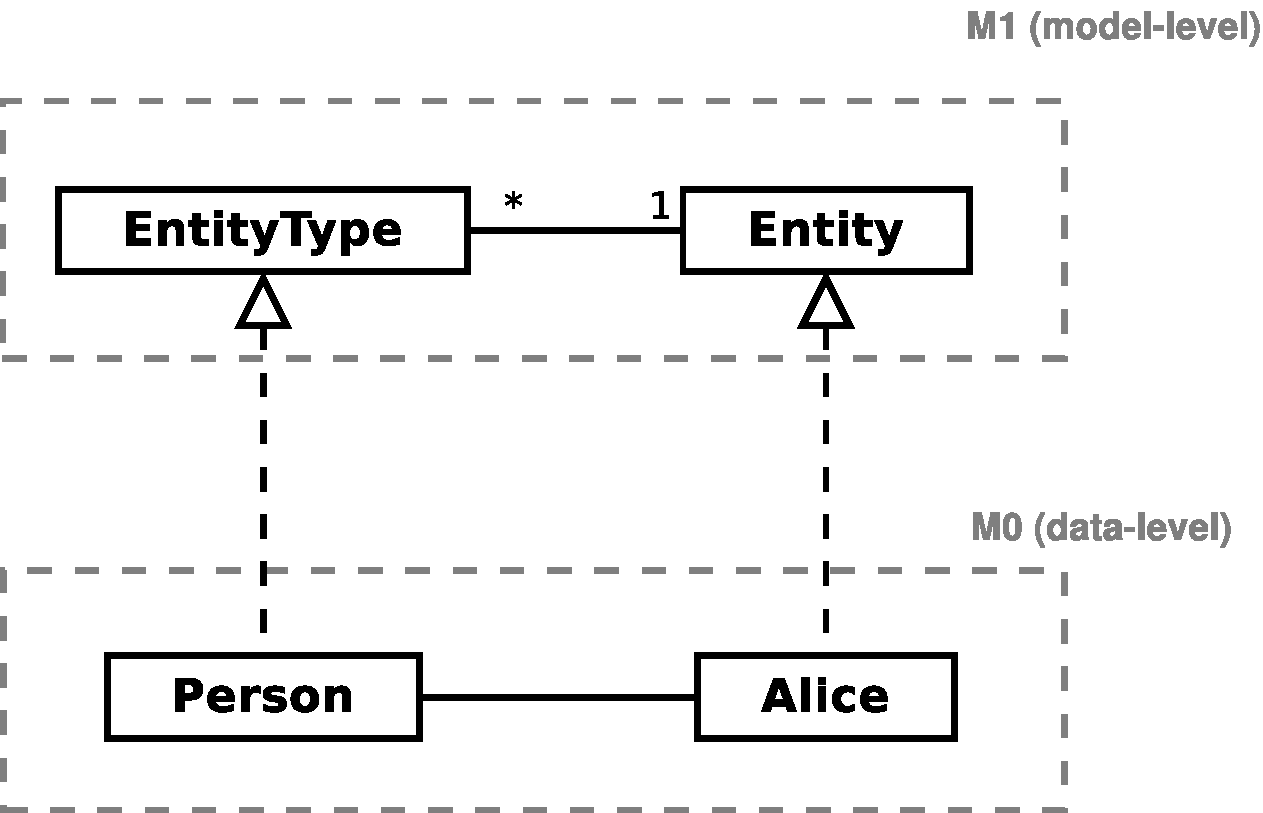
\includegraphics[width=75mm]{type_object.pdf}
  \caption{\textsc{type-object} pattern}
  \label{fig:type-object_pattern}
\end{figure}

\subsubsection{\textsc{Property} Pattern}\label{sec:property_pattern}

Similar to the problem solved by the \textsc{Type-Object}, the \textsc{property} pattern addresses the analogous issues of having the need to change the attributes of a class. The anticipation of these structural changes leads to the \textsc{property} pattern, where an attribute is split in two classes: the meta-class for the object to be created --- PropertyType, and an instance of that attribute --- Property. Fig. \ref{fig:property_pattern} represents the UML model for the \textsc{property} design pattern.

\begin{figure}[H]
  \centering
  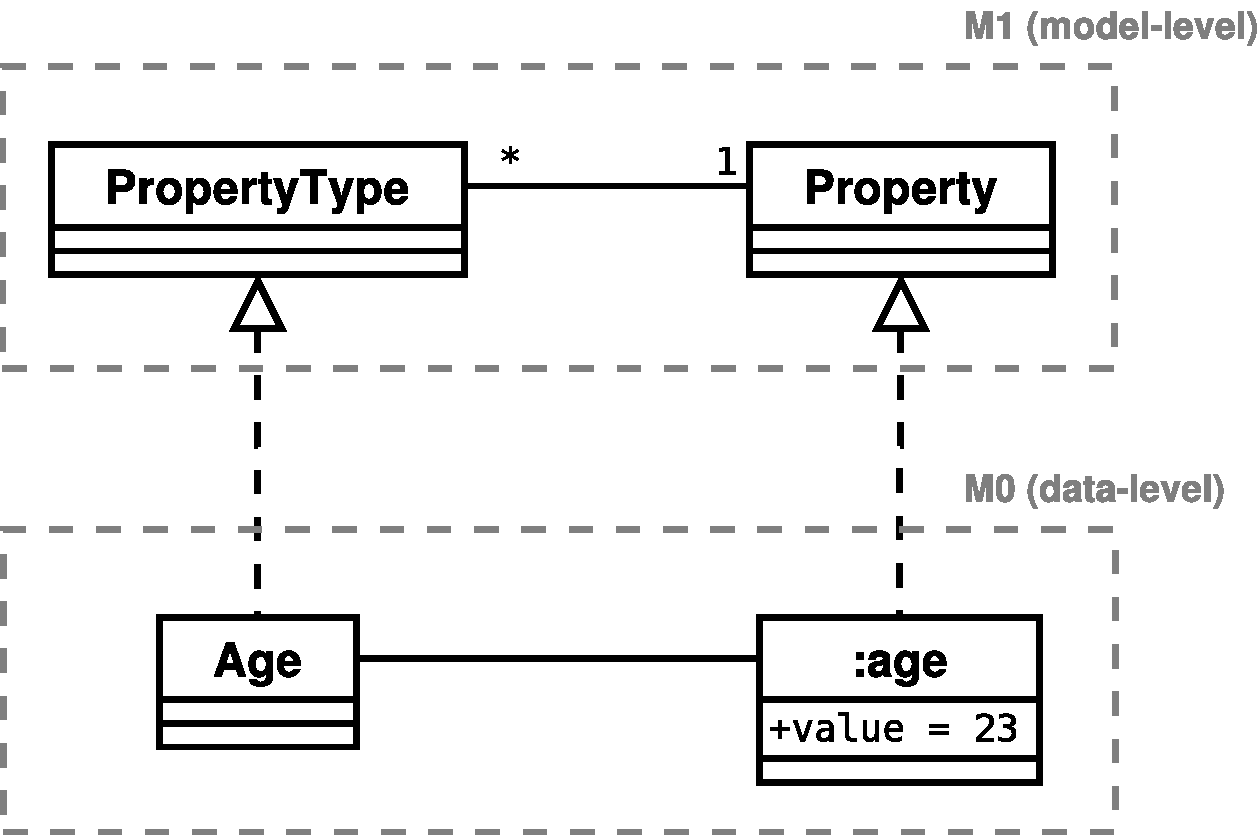
\includegraphics[width=80mm]{property}
  \caption{\textsc{property} pattern}
  \label{fig:property_pattern}
\end{figure}

\subsubsection{\textsc{Type-Square} Pattern}\label{sec:type-square_pattern}

Usually a class is modeled with a number of different attributes, representing their real world counterparts. So, in order to make a run-time modifiable class, an user must be able to modify both its \emph{definition} and \emph{attributes}. The answer to this issue is to use both \textsc{type-object} and \textsc{property} patterns at the same time, creating what is know as the \textsc{type-square} pattern --- which forms the basis of any AOM architecture \cite{YJ02}. Figure \ref{fig:type_square} shows the UML model for this pattern.

\begin{figure}[H]
  \centering
  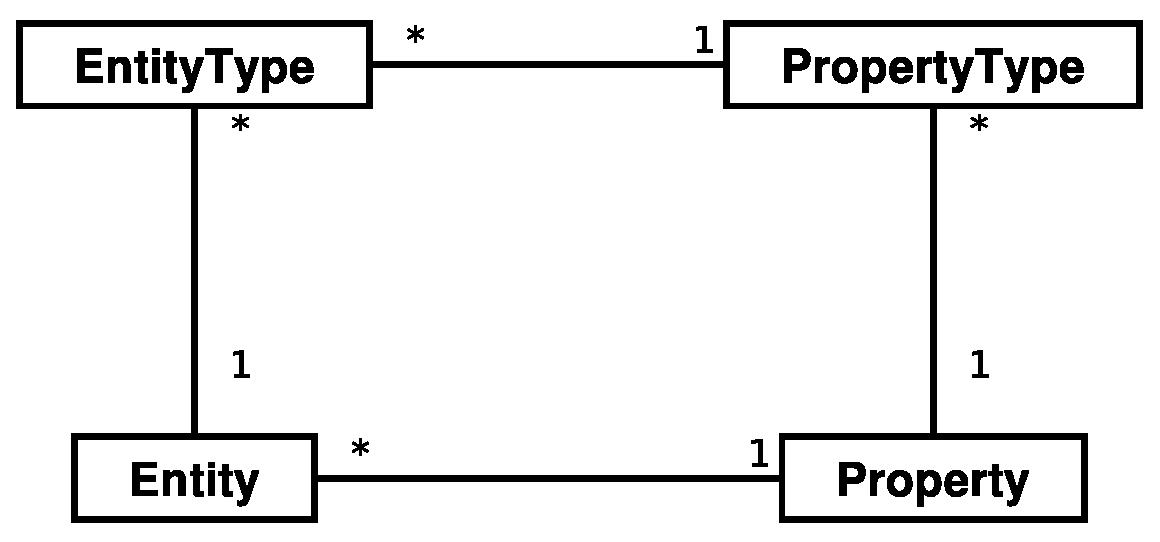
\includegraphics[width=90mm]{type_square}
  \caption{\textsc{type-square} pattern}
  \label{fig:type_square}
\end{figure}

\subsubsection{Relationships Between Entities}\label{sec:relationships_between_entities}

\cite{YJ02} describes the relationships between AOM classes by using the \textsc{accountability} pattern \cite{fowler, hay}.

Most OOP languages, however, describe object attributes as either primitive values or references to other objects. Some languages, such as Ruby and Smalltalk, treat everything as an object and do not make any difference between references and primitive values. These concepts can be used to extend the \textsc{property} pattern, and make it aware of relationships between entities, using attributes such as cardinality, navigability or role. \cite{aom_research_roadmap}. The revised \textsc{property} pattern is depicted in Figure \ref{fig:property_revised}:

\begin{figure}[H]
  \centering
  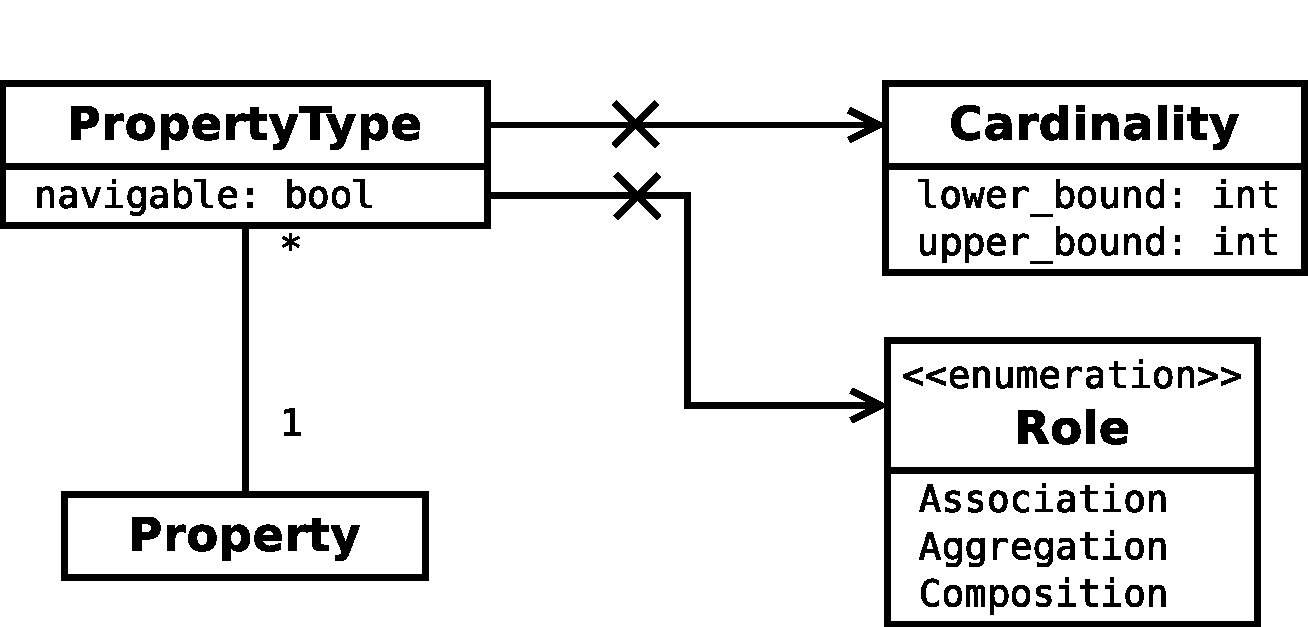
\includegraphics[width=100mm]{property_revised}
  \caption{Revised \textsc{property} pattern}
  \label{fig:property_revised}
\end{figure}

\section{Adaptability On The Web}\label{sec:web_adaptability}

Up until now, there has been very little work regarding adaptive systems on the web. There are a plethora of websites which offer varying degrees of customization, such as repositioning content on the webpage, or adding new content (usually small applications known as widgets), or changing the overall look of the application (more commonly known as \textit{skinning} or \textit{theming}) \cite{igoogle, pageflakes, protopage, webwag}.

Another approach taken to adaptability is to \emph{automatically} adapt to each individual user. This is accomplished by mining information relative to where the user comes from and its past actions in order to cater to the perceived results the user expected \cite{GGGR09}. As stated by \cite{NC}, 

\begin{quote}
  ``Adaptive software uses available information about changes in its environment to improve its behavior.''
\end{quote}

However, these websites do not allow their end users to modify the underlying \textit{model} of the system, only overall \textit{look \& feel} and, to some extent, functionalities --- which rely on the developers to be readily available.

As such these are not true \textit{adaptive systems} as per the definition gave by Joseph Yoder in \cite{YJ02}.

Nevertheless, these websites possess valuable information regarding the most commonly used user-interface mechanisms. Drag-and-drop is used extensively to reorganize information and perform basic tasks such as adding and removing basic container blocks.


